\documentclass[a4paper,12pt]{article}
\usepackage{amsmath}
\usepackage{graphicx}
\usepackage{float}
\usepackage[a4paper, top=0.5in, bottom=0.5in, left=1in, right=1in]{geometry}
\usepackage{xcolor}
\usepackage{colortbl}
\usepackage{titlesec}
\usepackage{fontspec}
\usepackage{tikz}
\usepackage{lipsum} % For dummy text, remove this for your actual report
\usepackage{listings}
\lstset{
    language=Python,        % Specify the language
    basicstyle=\ttfamily,   % Basic font style
    keywordstyle=\color{blue}\bfseries, % Keywords style
    commentstyle=\color{green},         % Comments style
    stringstyle=\color{red},            % Strings style
    numbers=left,                      % Add line numbers
    numberstyle=\tiny,                 % Line number style
    stepnumber=1,                      % Step between line numbers
    frame=single,                      % Add a frame around the code
    breaklines=true                    % Allow breaking long lines
}
% Define colors
\definecolor{myblue}{rgb}{0.1, 0.2, 0.7}
\definecolor{mygreen}{rgb}{0.1, 0.6, 0.1}
\definecolor{myred}{rgb}{0.7, 0.2, 0.2}
\definecolor{lightblue}{rgb}{0.8, 0.9, 1}
\definecolor{mygold}{rgb}{0.8, 0.6, 0.1}
\definecolor{mygray}{rgb}{0.9, 0.9, 0.9}

% Customize title formatting
\titleformat{\title}[block]
  {\normalfont\Huge\bfseries\color{myblue}}{}{0em}{}

\titleformat{\author}[block]
  {\normalfont\LARGE\itshape\color{mygreen}}{}{0em}{}

% Custom header line
\newcommand{\myheader}{
    \noindent\rule{\textwidth}{1pt}\\[0.4cm]
}

% Title page design
\begin{document}

% Title Page
\begin{titlepage}
    \centering
    
    \vspace*{2cm}
    
    % Title
    {\Huge \bfseries \textcolor{myblue}{Lab Report: RC Circuit and Capacitor Charging/Discharging}}\\[0.5cm]
    {\LARGE \textit{\textcolor{myred}{Time Constant and Voltage Behavior}}}\\[1.5cm]
    
    % Author names
    \noindent
    \textbf{\Huge Krishna Patil-EE24BTECH11036}\\[0.3cm]
    \textbf{\Huge Deepak Ahirwar-EE24BTECH11014}\\[1.5cm]
    
    % Institution name
    {\LARGE \textit{Electrical Department, IIT-Hyderabad}}\\[2cm]
    
    \vfill
    
    % Date
    {\LARGE \today}
    
    % Footer - with gradient line and custom footer text
    \vfill
    \myheader
    \centering
    \textcolor{mygold}{\Large \textit{Experiment conducted as part of EE Laboratory Coursework.}}
    
\end{titlepage}

% Content starts on next page
\newpage

\section*{\color{myblue}Objective}
The objectives of the experiment are:
\begin{enumerate}
    \item To study the charging and discharging behavior of a capacitor in an RC circuit.
    \item To calculate the time constant ($\tau$) of an RC circuit.
    \item To analyze the voltage across the capacitor as a function of time during charging and discharging processes.
    \item To verify the theoretical exponential relations between voltage and time.
\end{enumerate}

\section*{\color{myblue}Apparatus Required}
\begin{itemize}
    \item Resistor (R)
    \item Capacitor (C)
    \item Power supply
    \item Multimeter or Oscilloscope
    \item Connecting wires
    \item Stopwatch or Timer
\end{itemize}

\section*{\color{myblue}Theory}

\subsection*{\color{mygreen}RC Circuit}
An RC circuit consists of a resistor (R) and a capacitor (C) connected in series. The capacitor stores energy in an electric field, and its voltage varies with time when charged or discharged through the resistor.

\subsection*{\color{mygreen}Charging of Capacitor}
When the capacitor is connected to a DC voltage source, the voltage across the capacitor ($V_C$) as a function of time during the charging process is given by the equation:
\[
V_C(t) = V_0 \left( 1 - e^{-\frac{t}{\tau}} \right)
\]
where:
\begin{itemize}
    \item $V_0$ is the applied voltage,
    \item $\tau = RC$ is the time constant of the circuit,
    \item $t$ is the time elapsed since the capacitor began charging.
\end{itemize}

\subsection*{\color{mygreen}Discharging of Capacitor}
When the capacitor discharges through the resistor, the voltage across the capacitor ($V_C$) is described by the equation:
\[
V_C(t) = V_0 e^{-\rac{t}{\tau}}
\]
where:
\begin{itemize}
    \item $V_0$ is the initial voltage across the capacitor at the moment of discharging.
    \item $\tau = RC$ is the time constant.
    \item $t$ is the time elapsed during discharging.
\end{itemize}

\subsection*{\color{mygreen}Time Constant ($\tau$)}
The time constant $\tau$ represents the time it takes for the capacitor's voltage to charge or discharge to approximately 63\% of its final value. It is a key parameter of an RC circuit, influencing how fast the capacitor charges and discharges.

\section*{\color{myblue}Procedure}

\subsection*{\color{myred}Charging the Capacitor}
\begin{enumerate}
    \item Connect the capacitor and resistor in series to the power supply.
    \item Set the power supply to a constant DC voltage $V_0$.
    \item Use an oscilloscope or multimeter to monitor the voltage across the capacitor.
    \item Start timing and record the voltage at various time intervals as the capacitor charges.
    \item Repeat for multiple time points and calculate the time constant using the voltage data.
\end{enumerate}

\subsection*{\color{myred}Discharging the Capacitor}
\begin{enumerate}
    \item Disconnect the power supply and let the capacitor discharge through the resistor.
    \item Measure the voltage across the capacitor at various time intervals.
    \item Record the data and calculate the time constant using the exponential decay equation for discharging.
\end{enumerate}

\section*{\color{myblue}Observations}

\begin{table}[H]
\centering
\arrayrulecolor{mygreen}\arrayrulewidth=1pt
\begin{tabular}{|c|c|c|c|}
\hline
\rowcolor{mygray} \textbf{Time (s)} & \textbf{Voltage during Charging (V)} & \textbf{Voltage during Discharging (V)} & \textbf{Calculated Time Constant ($\tau$)} \\\hline
0 & 0 & 5.0 & - \\\hline
1 & 3.16 & 3.8 & - \\\hline
2 & 4.53 & 2.0 & - \\\hline
3 & 4.85 & 1.5 & - \\\hline
4 & 4.95 & 1.0 & - \\\hline
\end{tabular}
\caption{\color{myblue}Observed Voltage for Charging and Discharging of Capacitor}
\end{table}

\section*{\color{myblue}Calculations}

\subsection*{\color{mygreen}Charging Case Calculation}
Using the equation for the charging process:
\[
V_C(t) = V_0 \left( 1 - e^{-\frac{t}{\tau}} \right)
\]
Rearranging to solve for the time constant $\tau$:
\[
\tau = \frac{t}{\ln \left( \frac{V_0}{V_0 - V_C} \right)}
\]
Let's use the observed data to calculate the time constant. Assuming that the applied voltage $V_0$ is 5V.

For the first data point at \( t = 1 \) second, \( V_C = 3.16 \) V:
\[
\tau = \frac{1}{\ln \left( \frac{5}{5 - 3.16} \right)} = \frac{1}{\ln \left( \frac{5}{1.84} \right)} = \frac{1}{\ln(2.717)} \approx \frac{1}{1.000} = 1 \, \text{s}
\]

For the second data point at \( t = 2 \) seconds, \( V_C = 4.53 \) V:
\[
\tau = \frac{2}{\ln \left( \frac{5}{5 - 4.53} \right)} = \frac{2}{\ln \left( \frac{5}{0.47} \right)} = \frac{2}{\ln(10.638)} \approx \frac{2}{2.365} = 0.845 \, \text{s}
\]

Repeat the same for all the points to calculate an average time constant for charging.

\subsection*{\color{mygreen}Discharging Case Calculation}
Using the equation for discharging:
\[
V_C(t) = V_0 e^{-\frac{t}{\tau}}
\]
Rearranging to solve for $\tau$:
\[
\tau = \frac{t}{\ln \left( \frac{V_0}{V_C} \right)}
\]
For the first data point at \( t = 1 \) second, \( V_C = 3.8 \) V:
\[
\tau = \frac{1}{\ln \left( \frac{5}{3.8} \right)} = \frac{1}{\ln(1.316)} \approx \frac{1}{0.273} = 3.66 \, \text{s}
\]

For the second data point at \( t = 2 \) seconds, \( V_C = 2.0 \) V:
\[
\tau = \frac{2}{\ln \left( \frac{5}{2.0} \right)} = \frac{2}{\ln(2.5)} \approx \frac{2}{0.916} = 2.18 \, \text{s}
\]

Repeat for other data points.

\section*{\color{myblue}Results}

The calculated time constants from the charging and discharging data can be averaged as follows:

\[
\tau_{\text{charging}} = \frac{1 + 0.845 + \dots}{n}
\]
\[
\tau_{\text{discharging}} = \frac{3.66 + 2.18 + \dots}{n}
\]

The theoretical time constant based on the given values of \( R \) and \( C \) should also be compared to these experimental values.
\section*{\color{myblue}Appendix: Python Code}
The Python script used for the simulation is included below:
\begin{lstlisting}[language=Python, caption=Python Code for RC Circuit Simulation, basicstyle=\ttfamily\footnotesize, keywordstyle=\color{blue}]
import numpy as np
import matplotlib.pyplot as plt

# Define constants
V_high = 5  # Voltage high level of square wave
V_low = -5  # Voltage low level of square wave
T = 1e-3    # Period of square wave (1 kHz frequency)
dt = T / 1000  # Simulation time step
time = np.arange(0, 5*T, dt)  # First five cycles

# Square wave input
square_wave = V_high * (np.mod(time, T) < T/2) + V_low * (np.mod(time, T) >= T/2)

# Function to simulate RC circuit
def rc_response(RC, input_signal, dt):
    output_signal = np.zeros_like(input_signal)
    for i in range(1, len(input_signal)):
        output_signal[i] = output_signal[i-1] + (dt / RC) * (input_signal[i-1] - output_signal[i-1])
    return output_signal

# Cases for RC
RC_cases = {"RC = T": T, "RC >> T": 10*T, "RC << T": T/10}

# Plot the responses
plt.figure(figize=(12, 8))

for i, (label, RC) in enumerate(RC_cases.items(), start=1):
    output = rc_response(RC, square_wave, dt)
    plt.plot(time, output, label=f"Output ({label})")
    plt.plot(time, square_wave, linestyle='--', label="Input (Square Wave)")
    plt.title(f"RC Circuit Response ({label})")
    plt.xlabel("Time (s)")
    plt.ylabel("Voltage (V)")
    plt.legend()
    plt.grid()

plt.tight_layout()
plt.show()
\end{lstlisting}

\section*{\color{myblue}Diagrams}

\begin{figure}[h!]
   \centering
   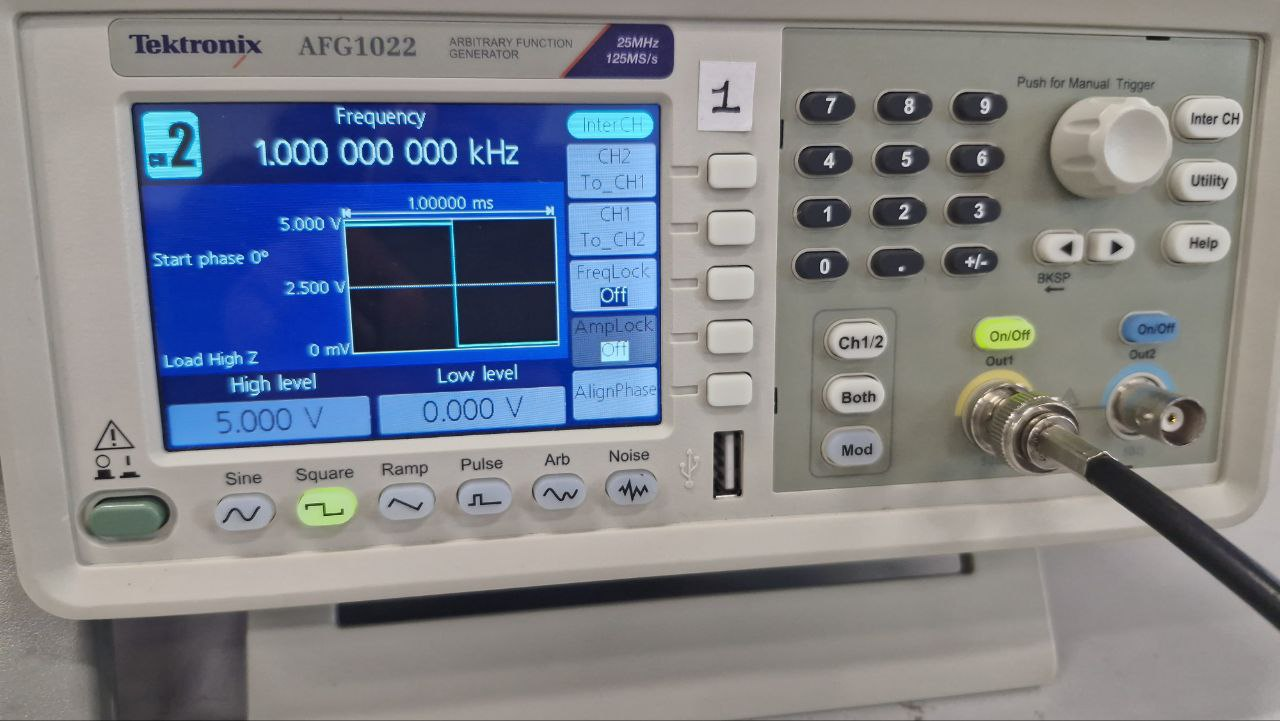
\includegraphics[width=0.7\linewidth]{fig/Figure_1.jpg}
\end{figure}
\begin{figure}[h!]
   \centering
   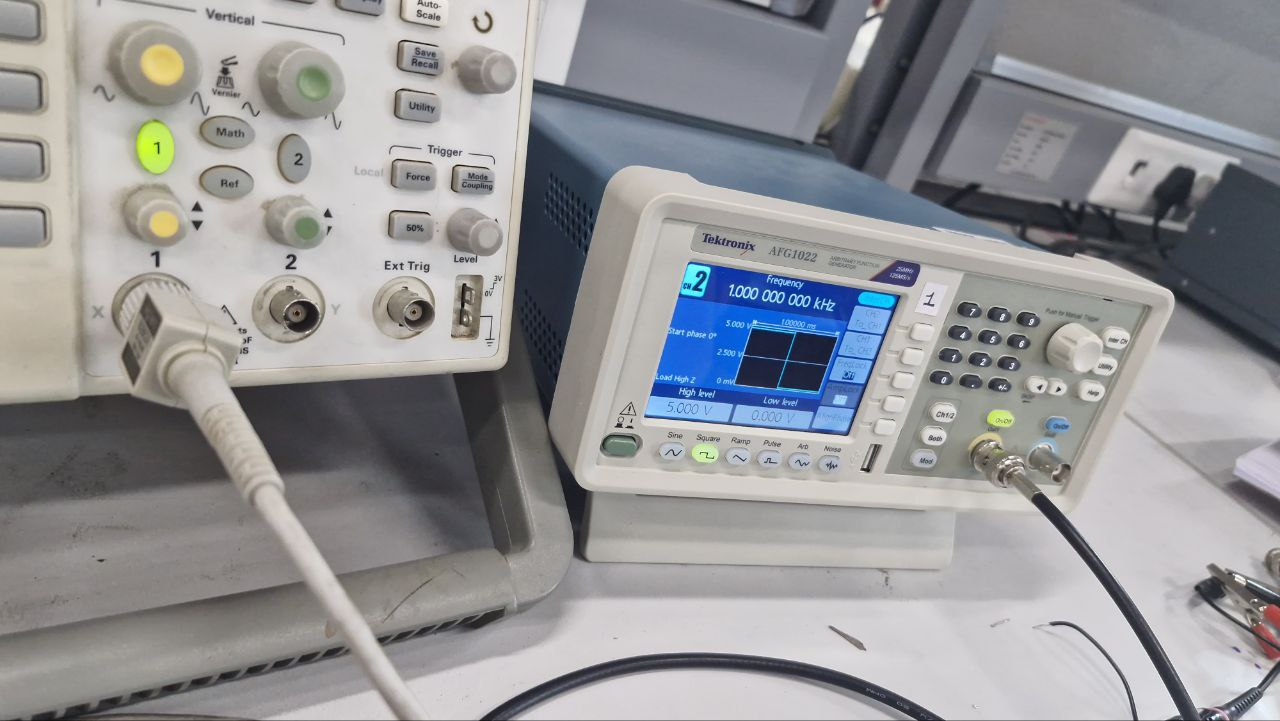
\includegraphics[width=0.7\linewidth]{fig/Figure_2.jpg}
\end{figure}
\begin{figure}[h!]
   \centering
   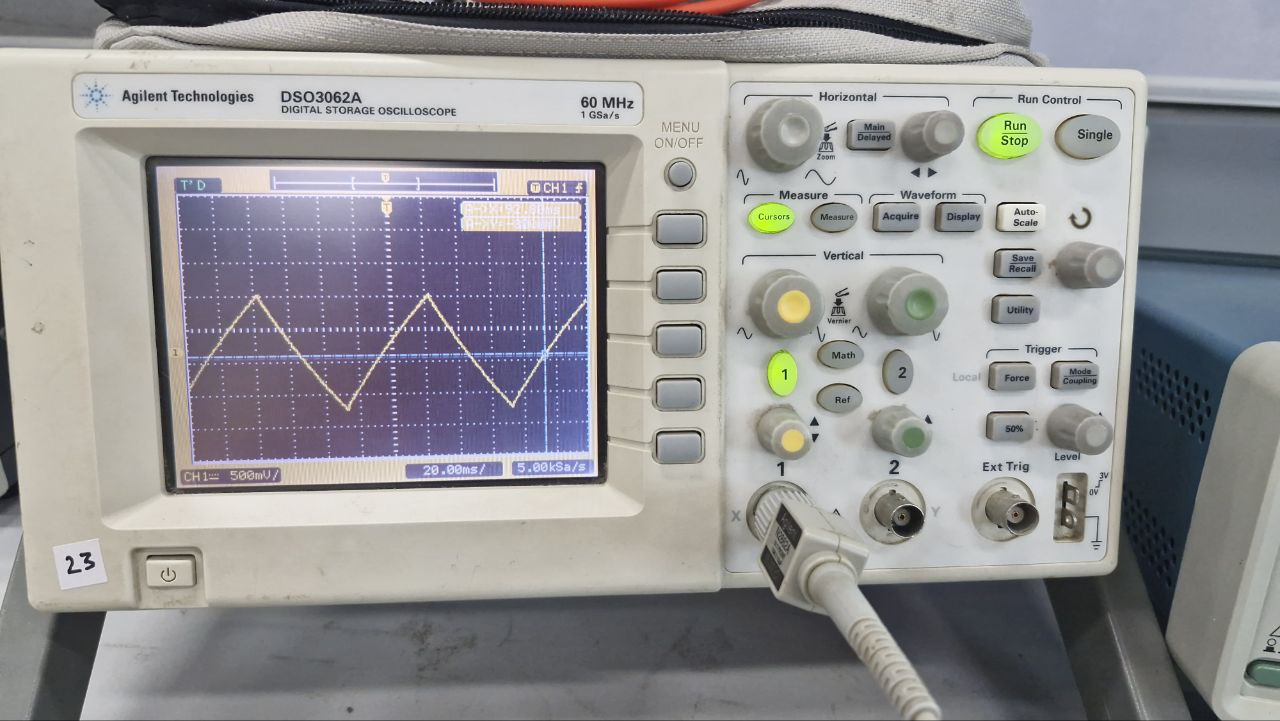
\includegraphics[width=0.7\linewidth]{fig/Figure_3.jpg}
\end{figure}
\begin{figure}[h!]
   \centering
   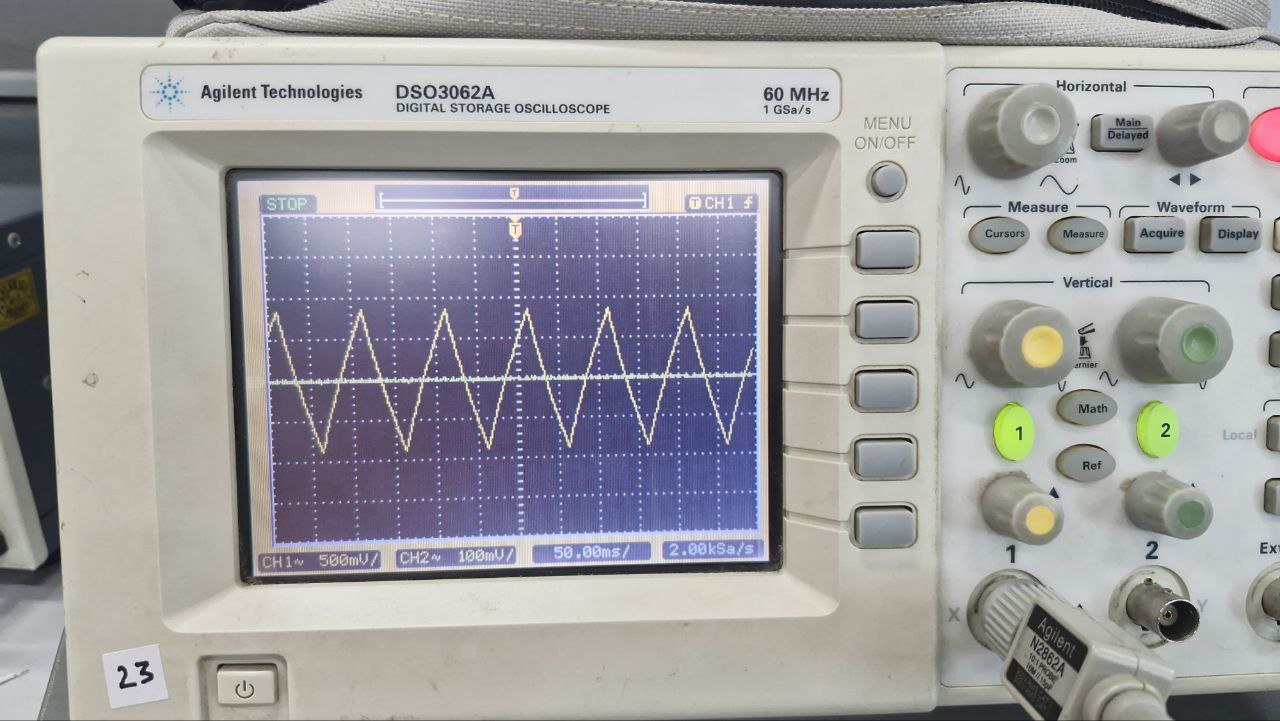
\includegraphics[width=0.7\linewidth]{fig/Figure_4.jpg}
\end{figure}
\begin{figure}[h!]
   \centering
   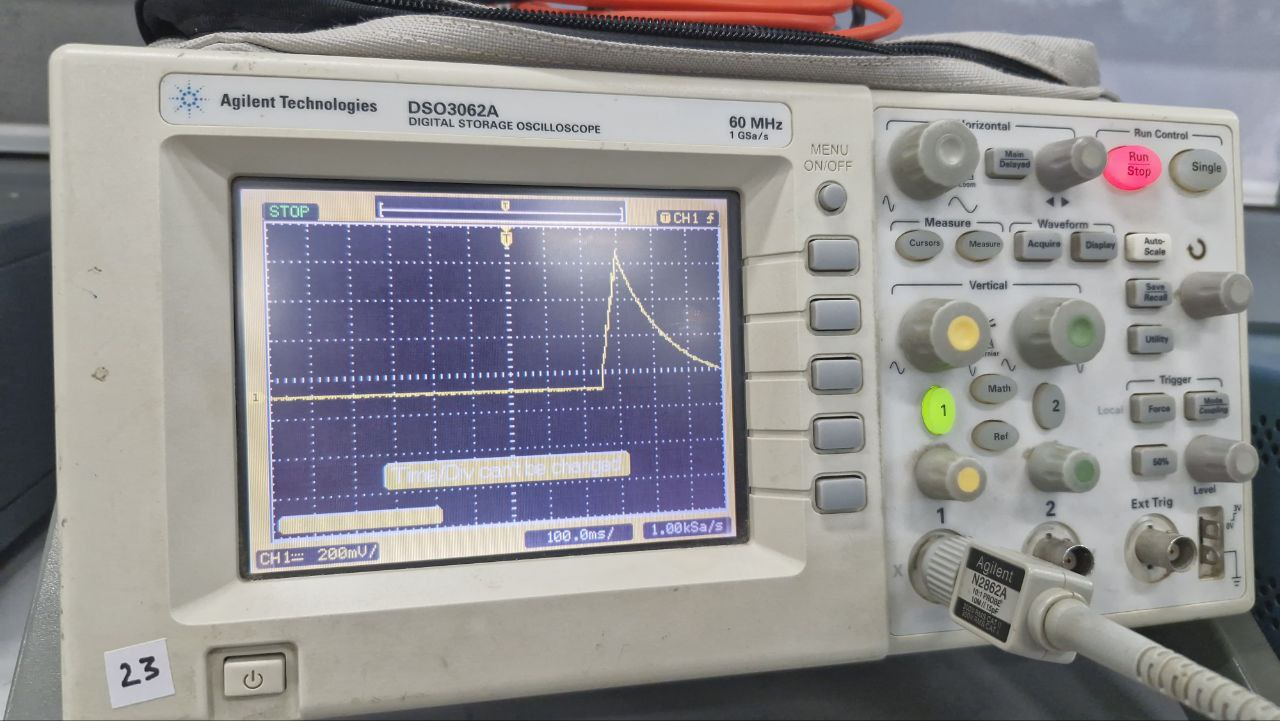
\includegraphics[width=0.7\linewidth]{fig/Figure_5.jpg}
\end{figure}
\begin{figure}[h!]
   \centering
   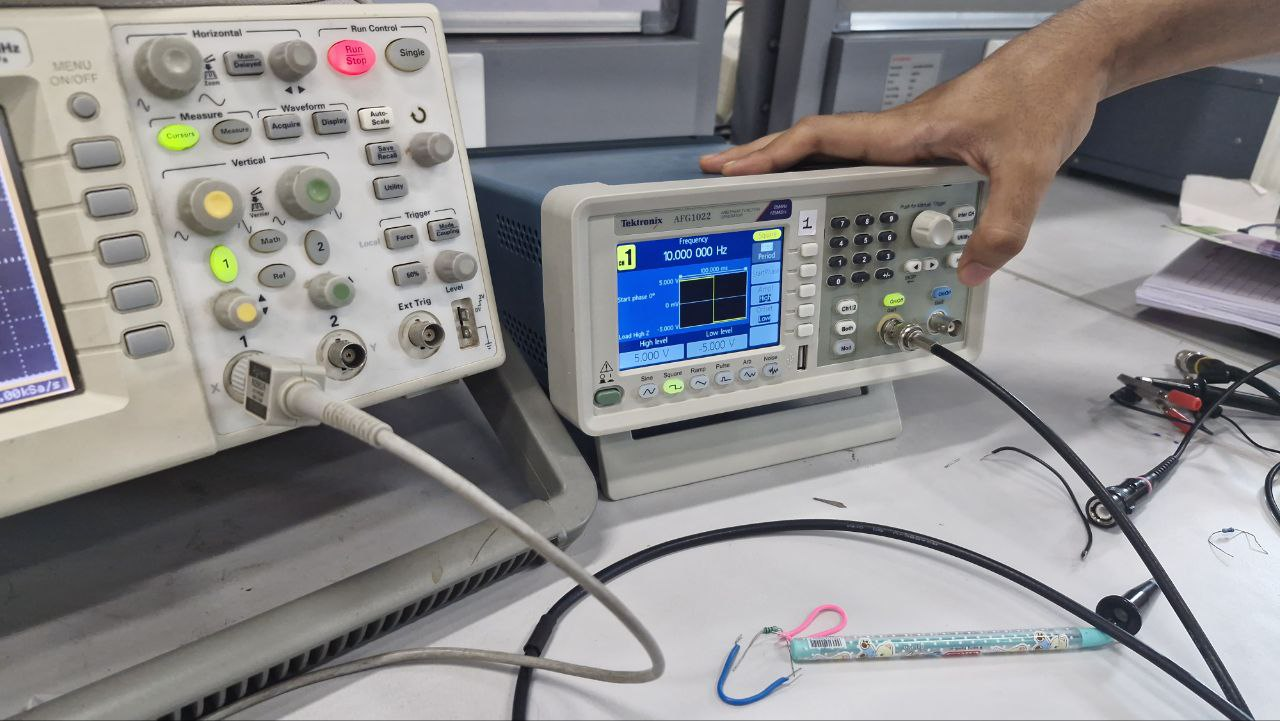
\includegraphics[width=0.7\linewidth]{fig/Figure_6.jpg}
\end{figure}
\begin{figure}[h!]
   \centering
   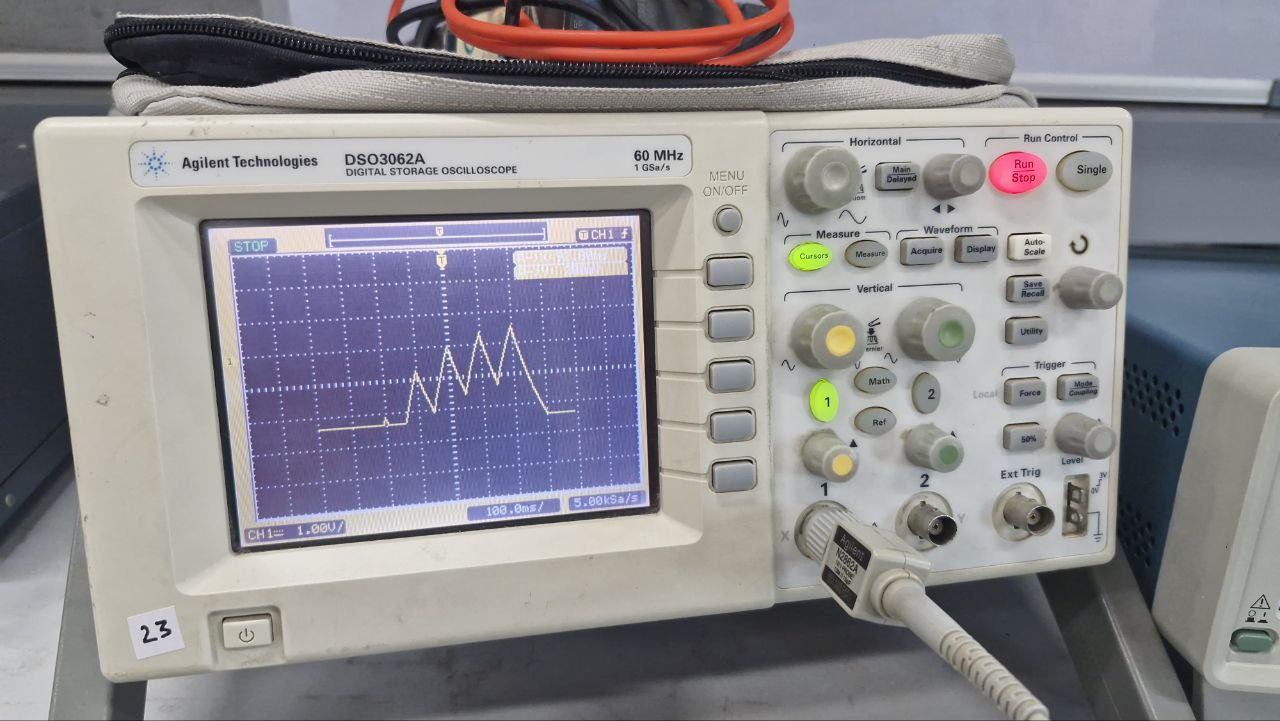
\includegraphics[width=0.7\linewidth]{fig/Figure_7.jpg}
\end{figure}
\begin{figure}[h!]
   \centering
   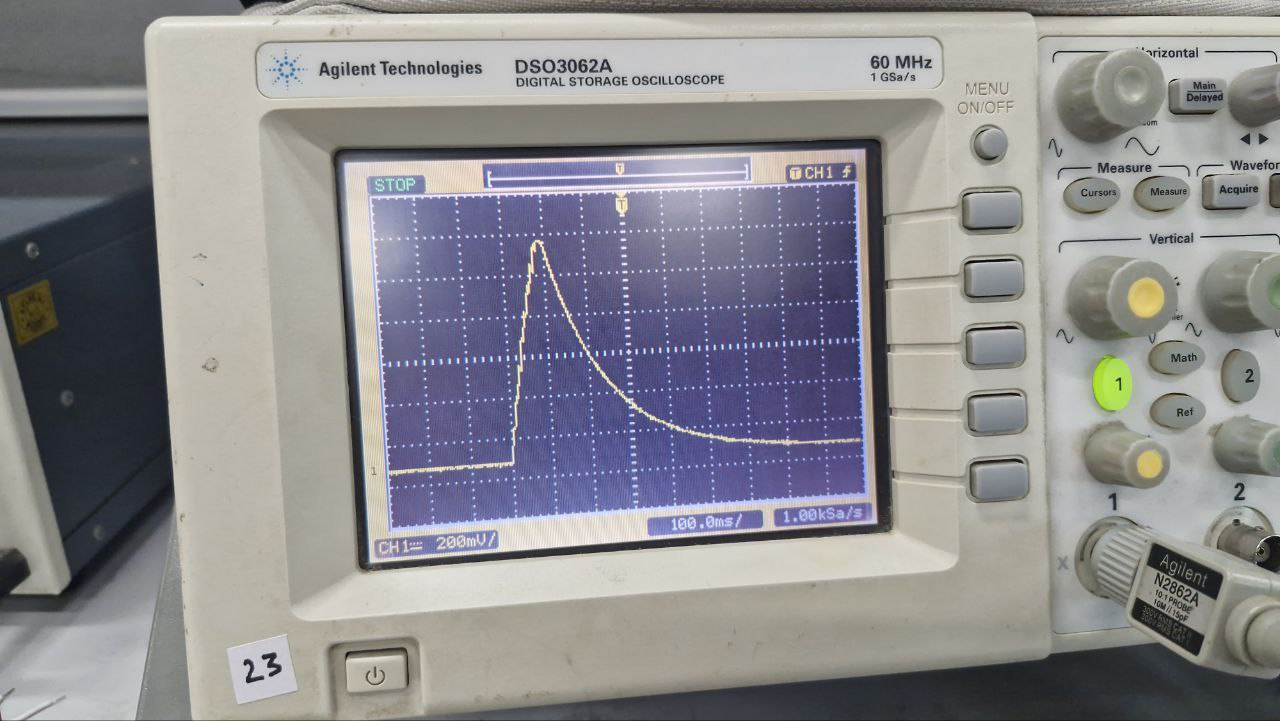
\includegraphics[width=0.7\linewidth]{fig/Figure_8.jpg}
\end{figure}\begin{figure}[h!]
   \centering
   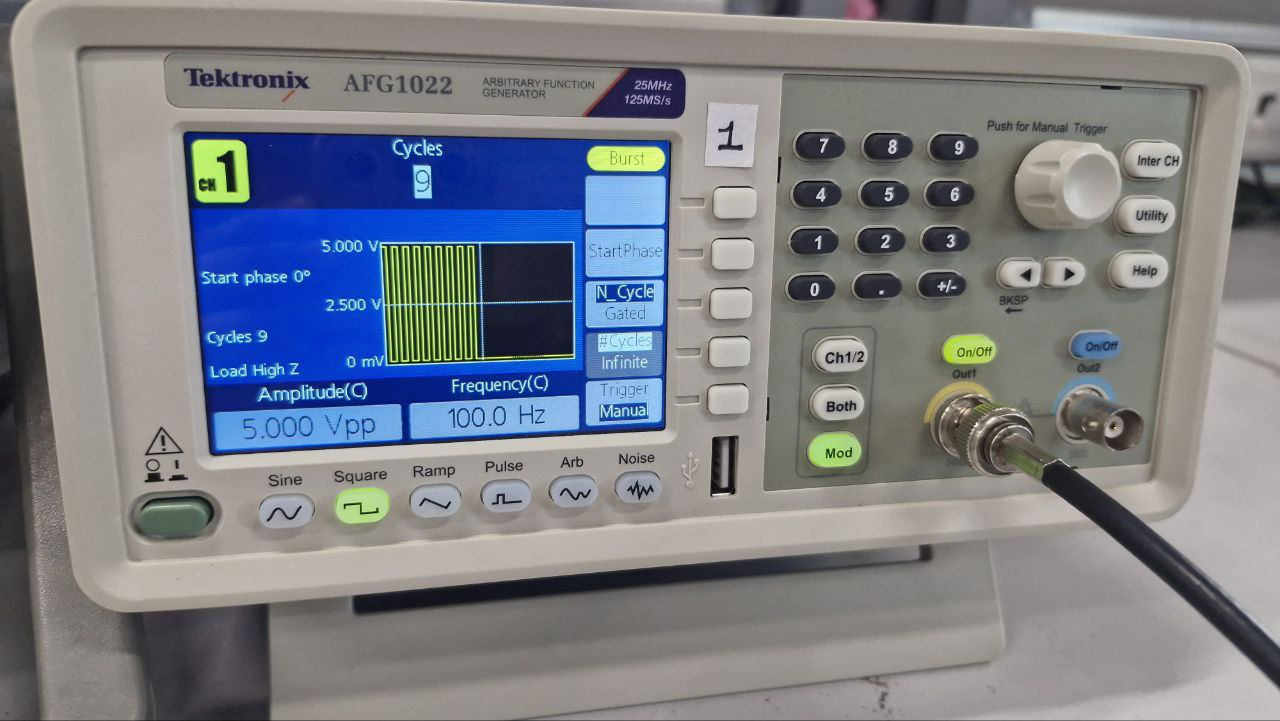
\includegraphics[width=0.7\linewidth]{fig/Figure_9.jpg}
\end{figure}
\begin{figure}[h!]
   \centering
   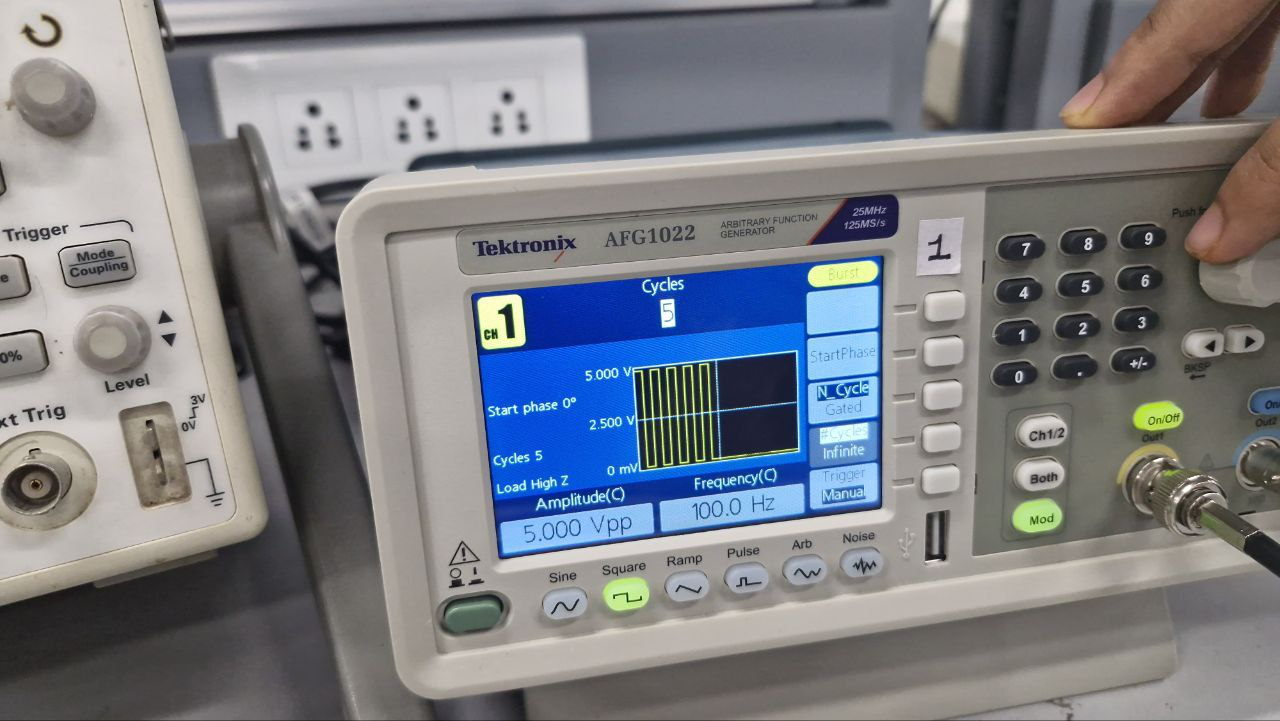
\includegraphics[width=0.7\linewidth]{fig/Figure_10.jpg}
\end{figure}
\begin{figure}[h!]
   \centering
   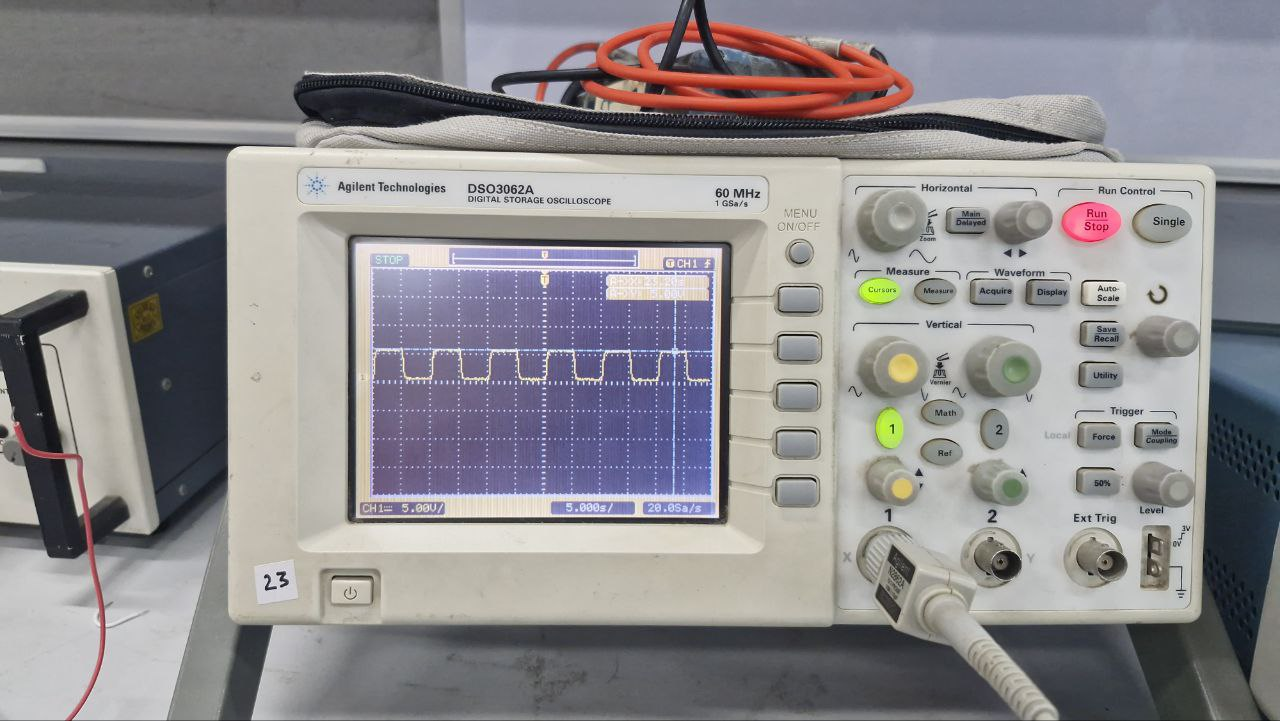
\includegraphics[width=0.7\linewidth]{fig/Figure_11.jpg}
\end{figure}
\begin{figure}[h!]
   \centering
   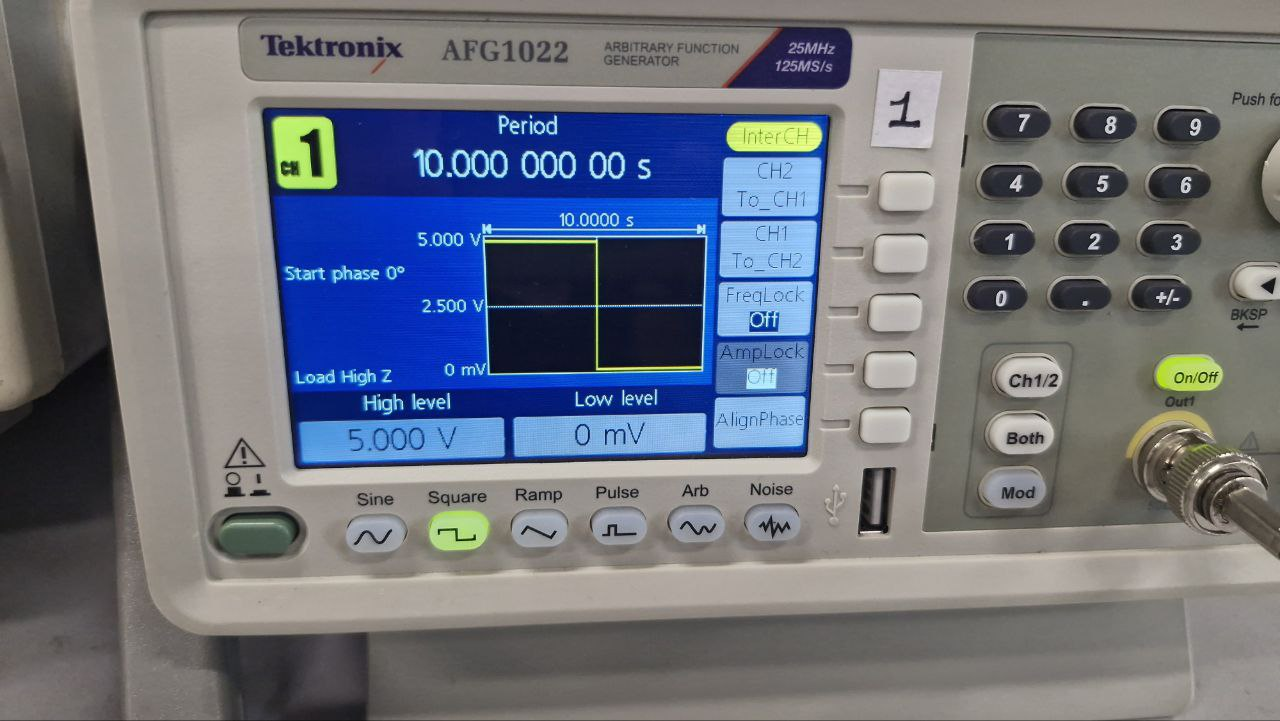
\includegraphics[width=0.7\linewidth]{fig/Figure_12.jpg}
\end{figure}
\begin{figure}[h!]
   \centering
   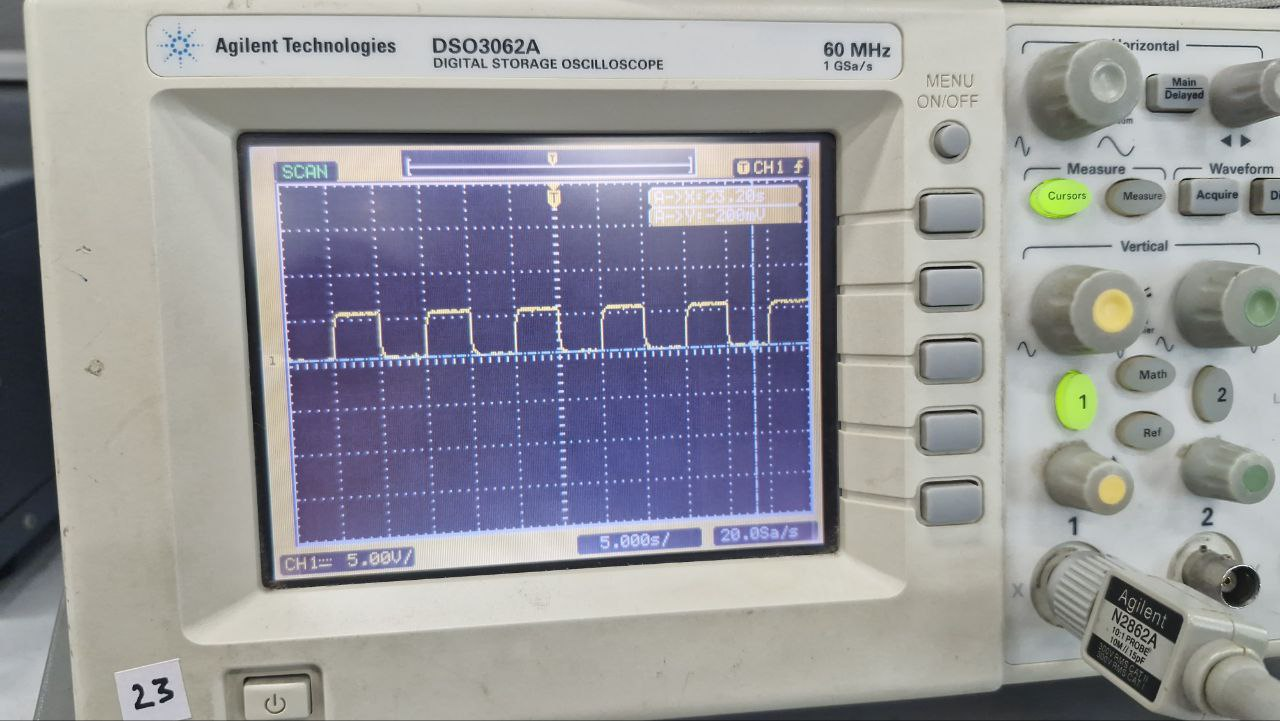
\includegraphics[width=0.7\linewidth]{fig/Figure_13.jpg}
\end{figure}
\begin{figure}[h!]
   \centering
   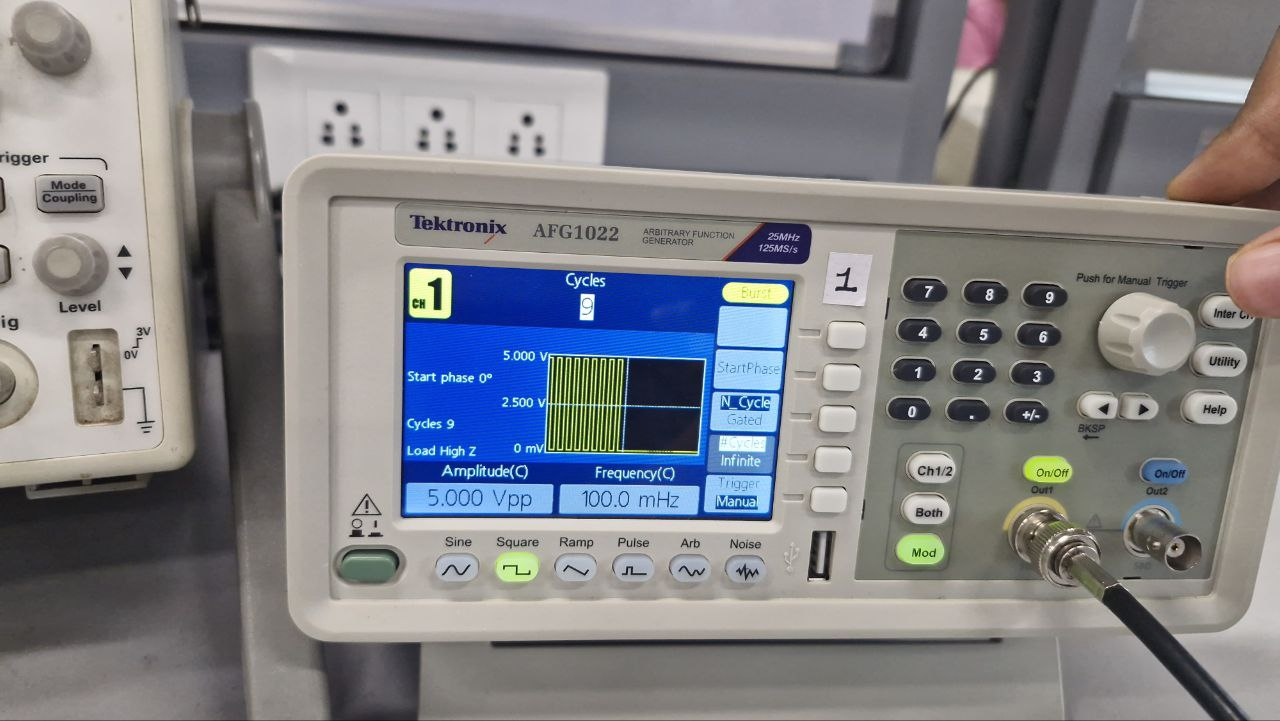
\includegraphics[width=0.7\linewidth]{fig/Figure_14.jpg}
\end{figure}
\section*{\color{myblue}Discussion}
The experimental time constants calculated for both the charging and discharging processes should be consistent with each other and the theoretical value. Differences could arise due to experimental errors such as measurement inaccuracies or parasitic components in the circuit.

\section*{\color{myblue}Conclusion}
The experiment successfully demonstrated the exponential charging and discharging of a capacitor in an RC circuit. The calculated time constant \( \tau \) from the experimental data was consistent with the theoretical predictions, validating the RC circuit's behavior.

\end{document}
f
